% Chapter Template

\chapter{Application et tests} % Main chapter title

\label{Chapter3} % Change X to a consecutive number; for referencing this chapter elsewhere, use \ref{ChapterX}


\lhead{Chapter 3. \emph{Application et tests}} % Change X to a consecutive number; this is for the header on each page - perhaps a shortened title


%----------------------------------------------------------------------------------------
%	SECTION 1
%----------------------------------------------------------------------------------------

\section{Introduction}

Nous présentons dans ce  chapitre les résultats de notre application et leur intérpertation. Ainsi que les détails des fonctionnalités disponibles.

%-----------------------------------
%	SECTION 2
%-----------------------------------
\section{Outils utilisés}

\indent Nous avons choisi comme langage de programmation le langage Python2.7 et ce pour diverses raisons dont on site [HOY 10]:\\

\begin{itemize}
\item Facilité d’écriture et de compréhension du code. On trouve moins de barrière entre la génération d'idée, et leurs traduction en code.
\item Balance entre langage de haut et de bas niveau. Ce qui forme un point fort du langage.
\item L'interopérabilité avec les autres langages, ou la capacité très utile à pouvoir appeler des script d'autres langages facilement.
\item Le grand nombre de bibliothèques disponibles.
\item La documentation abondante.\\
\end{itemize}

\indent Le traitement bas niveau des images se fait avec la bibliothèque graphique libre OpenCV qui propose un bon nombre de fonctions permettant d'effectuer les opérations classiques.\\

\indent Nous avons choisi d'utiliser pour le développement de l'interface graphique le framework PyQt, un module qui permet de lier le langage Python avec la bibliothèque Qt. En utilisant l'environnement \textit{Qt4 Designer version 4.8.1}.\\

Pour améliorer la vitesse de découpage, il s'est avéré qu'appeler un script matlab est bien plus intéressant en terme de temps d’exécution que de reprogrammer le script en python. La version de matlab utilisée étant \textit{R2012a 7.14.0.739 32-bit(glnx86)} \\

Ce document est rédigé en \textit{Latex}, avec \textit{Texmaker 3.2}.

%----------------------------------------------------------------------------------------
%	SECTION 3
%----------------------------------------------------------------------------------------
\section{Presentation et test de l'application:}

Nous commençons par exécuter l'application. [Figure 3.1]

Elle nous permet de choisir une image en cliquant sur Browse pour parcourir nos fichiers, ou en collant directement son chemin absolu.\\
Nous choisissons ensuite la valeur du \textit{threshold}.

\begin{figure}[H]
	\centering
		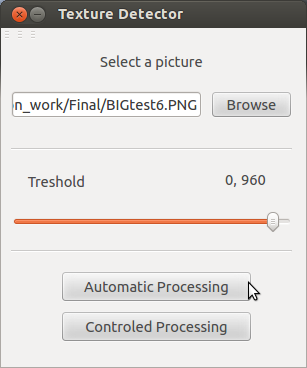
\includegraphics[width=7cm,]{Figures/chap3/3.png}
			\caption[choice1]{Fenêtre principale.}
	\label{fig:choice1}
\end{figure}

\indent Nous avons après cela le choix entre deux méthodes: 
\begin{itemize}


\item Automatic Processing: qui fait un traitement automatique des textures \\
\item Controled Processing: qui permet d'avoir plus de contrôle sur le traitement et la reconnaissance des textures. Il est aussi considéré comme processus d’entraînement de l'analyseur.\\
\end{itemize}
\indent Nous commençons par le traitement automatique. La fenêtre de la figure 3.2 nous est affiché, elle montre à droite l'image sélectionnée et en bas le \textit{threshold}, avec possibilité de les modifier.

\begin{figure}[H]
	\centering
		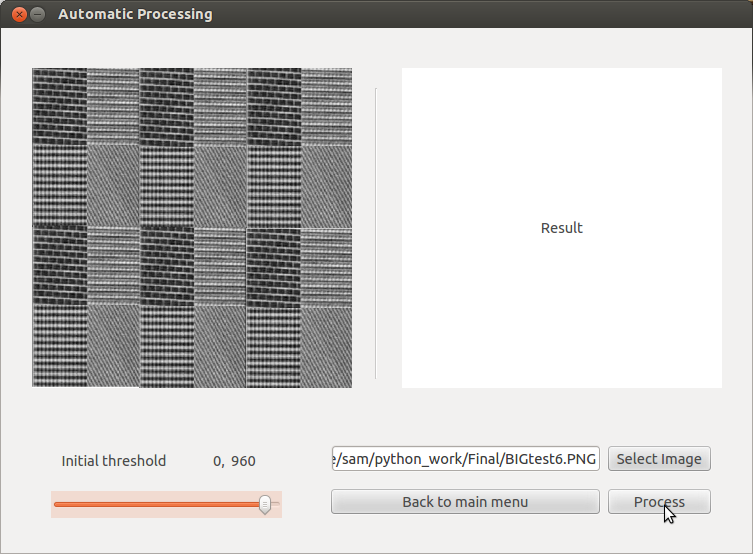
\includegraphics[width=12cm,]{Figures/chap3/4.png}
	\caption[traitementAuto]{Traitement automatique.}
	\label{fig:traitementAuto}
\end{figure}

\indent Nous cliquons sur \textit{Process} pour lancer le traitement.
Après quelques instants, le résultat de la détection et coloration des textures nous est affiché à droite de la fenêtre. [Figure 3.3]

\begin{figure}[H]
	\centering
		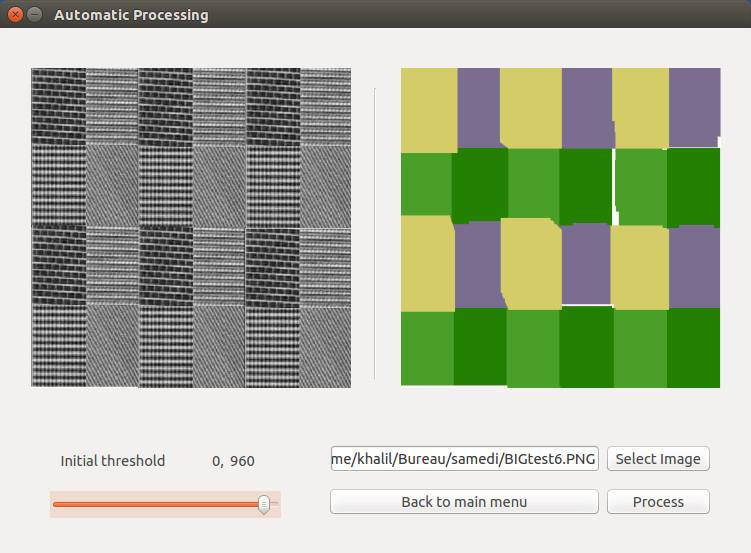
\includegraphics[width=12cm,]{Figures/chap3/5.jpg}
	\caption[traitementAutofin]{Traitement automatique fini.}
	\label{fig:traitementAutofin}
\end{figure}

\indent L'image résultante est automatiquement enregistrée dans le dossier contenant l'application. Comme expliqué dans le précédent chapitre, les \textit{thresholds} utilisés pour les différentes textures détectées sont tirés d'une base de données remplit à chaque usage du traitement contrôlé.

\indent Nous revenons vers le menu principale en cliquant sur le bouton \textit{Back to main menu}, et nous choisissons cette fois \textit{Controled Processing}.
Nous allons tester le traitement contrôlé où nous allons pouvoir modifier à chaque fois le \textit{threshold} de chaque texture détectée. Nous changerons aussi les informations présente dans la base de donnée en sauvegardant les résultats satisfaisants des détections d'une texture x.\\
\indent Prenons l'exemple de la figure 3.4. La première étape étant identique au traitement automatique, nous choisissons l'image et un \textit{threshold} par défaut. Nous commençons le traitement en cliquant sur \textit{Proces}.


\begin{figure}[H]
	\centering
		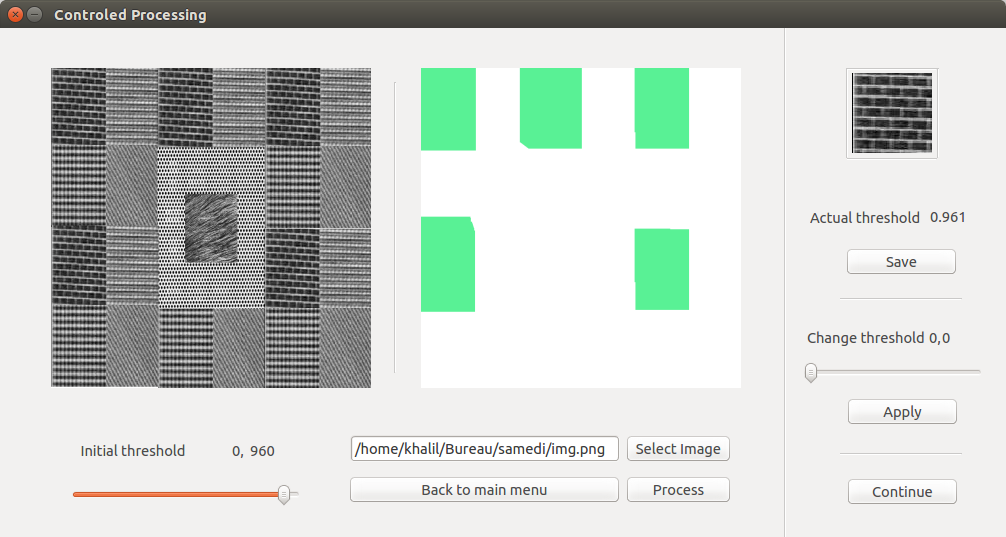
\includegraphics[width=15cm,]{Figures/chap3/Capture4343.png}
	\caption[traitementAutofin]{Traitement contrôlé - Itération 1.}
	\label{fig:traitementAutofin}
\end{figure}


\indent Une première texture est détectée, et les régions ressemblantes à cette dernière sont coloriées. Remarquons que le \textit{threshold} utilisé (\textit{Actual threshold 0.961}) est différent de celui choisi pour être par défaut (\textit{Initial threshold 0.960}). Ceci est du au fait que la même texture, ou une texture fortement ressemblante ai été trouvé dans la base de donnée. Le \textit{threshold} de cette dernière a été donc choisi.

\indent Nous avons, ensuite, la main pour choisir de sauvegarder le \textit{threshold} dans la base de donnée, de continuer si le résultat est satisfaisant, ou de changer ce premier et rechercher les zones ressemblantes à la texture détectée à nouveau.

\indent Nous choisissons de continuer, jusqu'a ce que l'a détection de l'une des textures n'est pas satisfaisante. Nous choisissons dans ce cas de changer le \textit{threshold}.[Figure 3.5]


\begin{figure}[H]
	\centering
		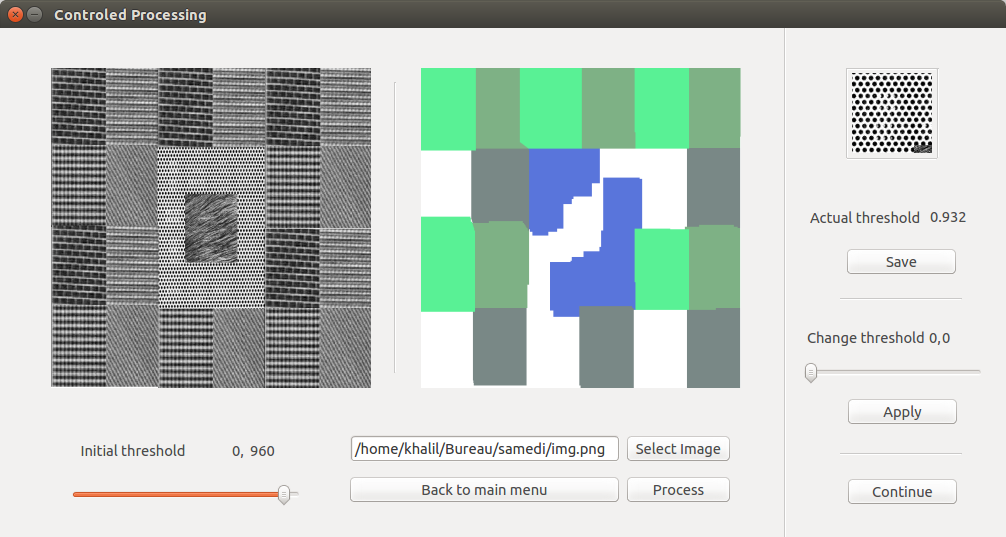
\includegraphics[width=15cm,]{Figures/chap3/Capture4826.png}
	\caption[traitementAutofin]{Traitement contrôlé - Itération 4.}
	\label{fig:traitementAutofin}
\end{figure}

Nous cliquons sur apply pour cela après avoir choisi un nouveau \textit{threshold} dans la partie \textit{Change threshold} [Figure 3.6].

\begin{figure}[H]
	\centering
		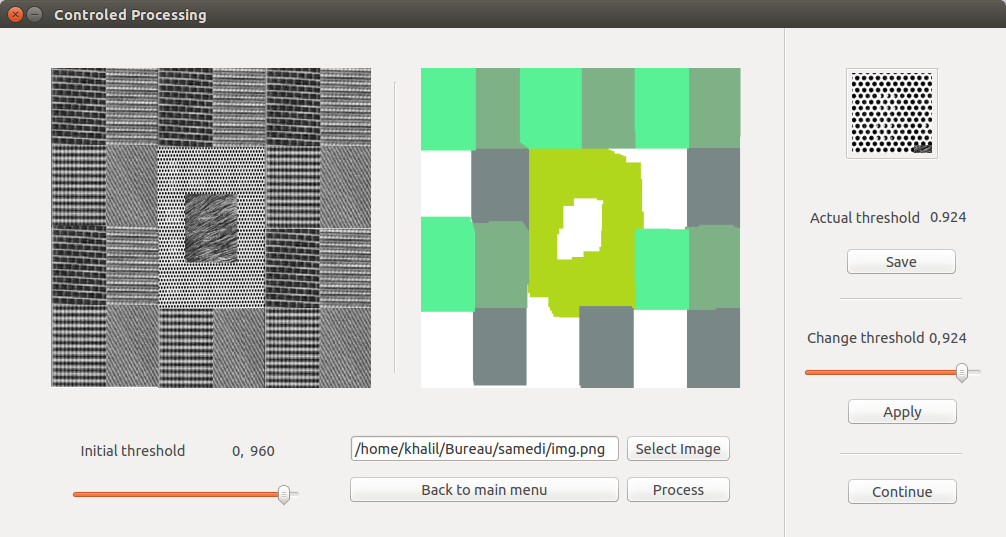
\includegraphics[width=15cm,]{Figures/chap3/Capture5010.png}
	\caption[traitementAutofin]{Traitement controlé - Itération 5.}
	\end{figure}

\indent Nous allons sauvegarder ce \textit{threshold} dans la base de donnée en appuyant sur le bouton \textit{Save} pour que la prochaine fois cette valeur sera utilisé automatiquement.

Le processus continue de la sorte jusqu’à ce que toutes les textures de l'image soient détectées [Figure 3.7].


\begin{figure}[H]
	\centering
		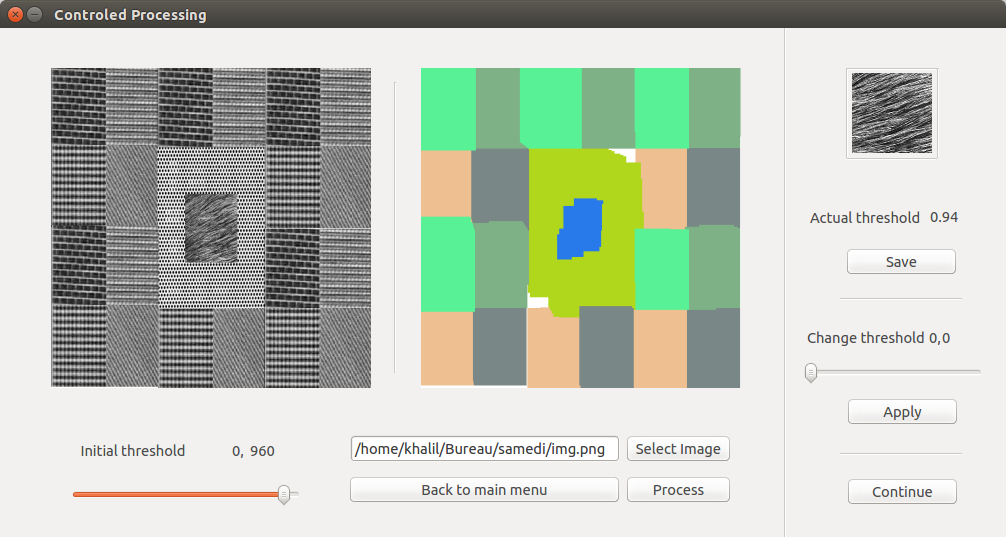
\includegraphics[width=15cm,]{Figures/chap3/Capture5253.png}
	\caption[traitementAutofin]{Traitement contrôlé - Itération 7.}
\end{figure}

\section{Tests et intérpretation des résultats:}

Nous allons voir plus en détails les résultats de plusieurs tests pour voir le comportement du threshold vis-à-vis des différentes textures.\\

Les détails des threshold choisi pour les textures détectés et leur surface occupé dans l'image (par carré de 150*150 px) sont représentés dans le tableau suivant .\\



%----------------- PREMIER TESTE ----------------------------------
\begin{figure}[htbp]
\centering
\begin{tabular}{cc}
\centering
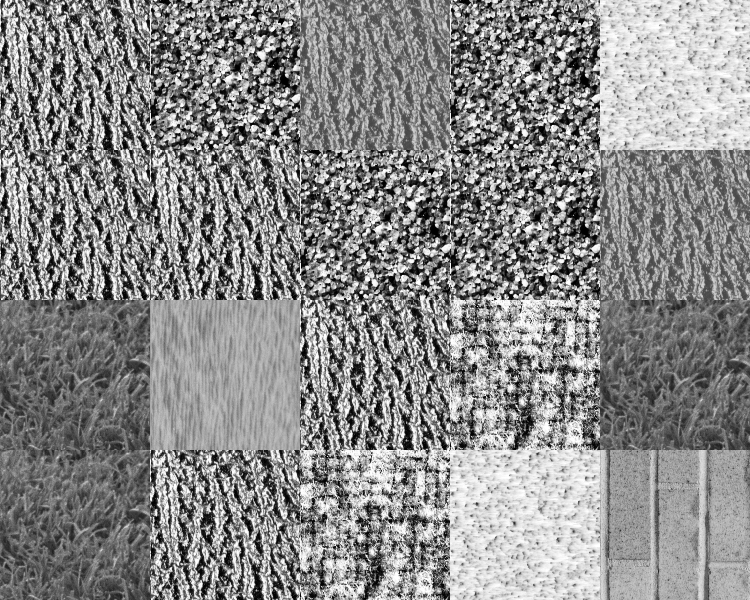
\includegraphics[width=6cm,]{Figures/chap3/texture1.png}
&

\includegraphics[width=6cm,]{Figures/chap3/texture1c.png}\\
&
\end{tabular}
\caption[test1]{Test 1\\}
\end{figure}

\begin{center}
\begin{tabular}{ | c c c | }
	\hline                       
	texture & surface (par carré) & threshold\\
	\hline                       
	  1 & 2 & 0,969    \\
	  2 & 3 & 0.997  \\
	  3 & 4 & 0.973  \\
  	  4 & 2 & 0.971 \\
	  4 & 3 & 0.964\\
	  6 & 1 & 0.964 \\
	\hline                       
\end{tabular}
\end{center}

%----------------- DEUXIEME TESTE ----------------------------------

\begin{figure}[htbp]
\centering
\begin{tabular}{cc}
\centering
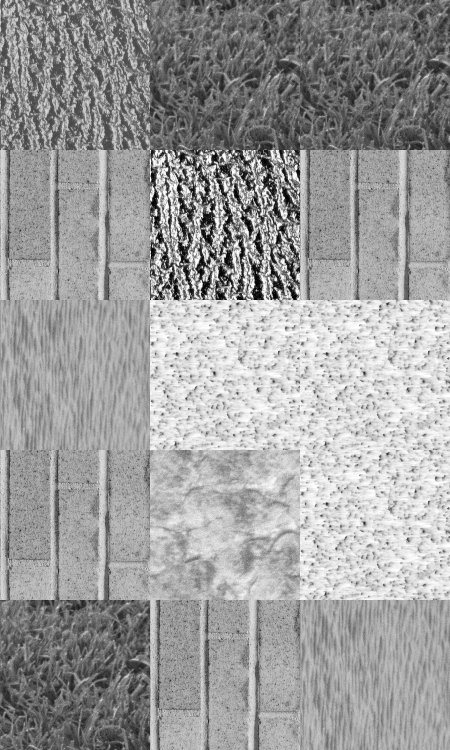
\includegraphics[width=6cm,]{Figures/chap3/texture2.png}
&

\includegraphics[width=6cm,]{Figures/chap3/texture2c.png}\\
&
\end{tabular}
\caption[test2]{Test 2\\}
\end{figure}

\begin{center}
\begin{tabular}{ | c c c | }
	\hline                       
	texture & surface (par carré) & threshold\\
	\hline                       
	  1 & 7 & 0,972    \\
	  2 & 4 & 0.971  \\
	  3 & 2 & 0.969  \\
  	  4 & 3 & 0.970 \\
	  5 & 1 & 0.976\\
	  6 & 2 & 0.958 \\
  	  7 & 2 & 0.973 \\
	\hline                       
\end{tabular}
\end{center}

%----------------- TROISIEME TESTE ----------------------------------

\begin{figure}[htbp]
\centering
\begin{tabular}{cc}
\centering
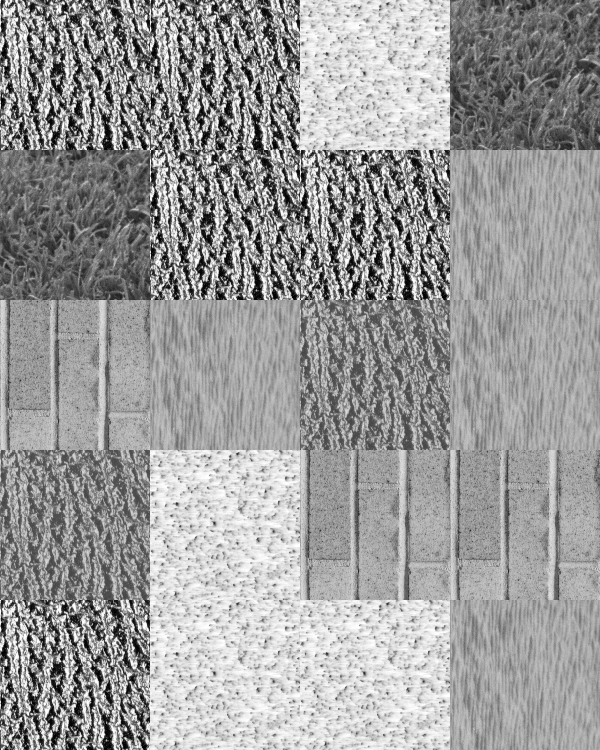
\includegraphics[width=6cm,]{Figures/chap3/texture3.png}
&

\includegraphics[width=6cm,]{Figures/chap3/texture3c.png}\\
&
\end{tabular}
\caption[test3]{Test 3\\}
\end{figure}

\begin{center}
\begin{tabular}{ | c c c | }
	\hline                       
	texture & surface (par carré) & threshold\\
	\hline                       
	  1 & 7 & 0,972    \\
	  2 & 4 & 0.972  \\
	  3 & 2 & 0.965  \\
  	  4 & 4 & 0.958 \\
	  5 & 3 & 0.973\\
	\hline                       
\end{tabular}
\end{center}


%-------------------- MOYENNE -------------------------

\paragraph*{}
Nous avons fait une dizaine de tests similaires. Nous avons calculé les moyenne des treshold par image dans un premier lieu, et puis, nous avons pris en compte les coefficients en fonction de la surface qu'ils occupent dans l'image. \\

Les résultats sont représentés dans le graphe suivant:

Graph représentatifs des moyenes.

\paragraph*{}
Nous remarquons que, malgré la différence considérable entre les thresholds des différentes textures, la moyenne entre ces derniers restes constante. Et ce, que ce soit avec ou sans compter le coéfficient relative à la surface occupée par les textures. 

Ceci implique que la précision en terme de détection reste élevée.


\subsection{Tests suplémentaires}

\begin{figure}

\begin{tabular}{cccc}


\multicolumn{2}{c}{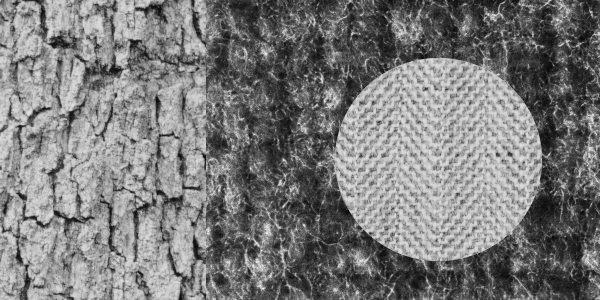
\includegraphics[width=8cm, height=4cm]{Figures/chap3/cercle1.png}}
&
\multicolumn{2}{c}{
\includegraphics[width=8cm, height=4cm]{Figures/chap3/cercle1cc.png}}\\

\multicolumn{4}{c}{(a) Image avec cercle}\\


\multicolumn{2}{c}{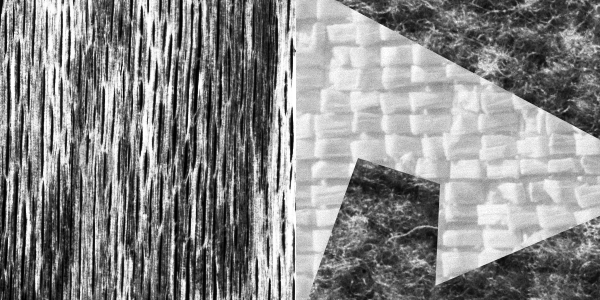
\includegraphics[width=8cm, height=4cm]{Figures/chap3/randome1.png}}
&
\multicolumn{2}{c}{
\includegraphics[width=8cm, height=4cm]{Figures/chap3/randome1cc.png}}\\

\multicolumn{4}{c}{(b) Image aléatoire 1}\\


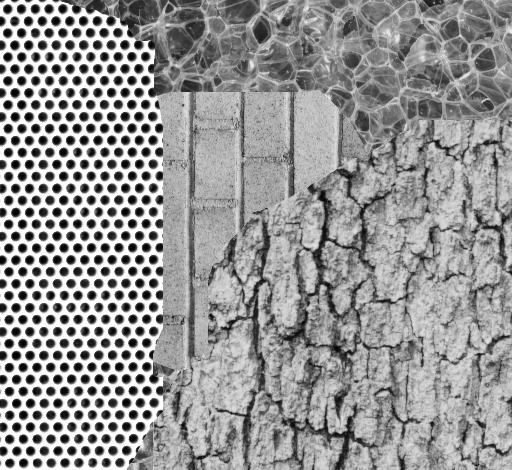
\includegraphics[width=4cm, height=4cm]{Figures/chap3/first.png}
&

\includegraphics[width=4cm, height=4cm]{Figures/chap3/first2.png}
&
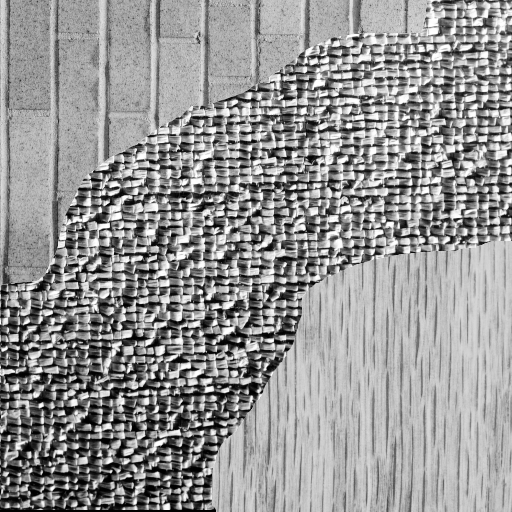
\includegraphics[width=4cm, height=4cm]{Figures/chap3/second.png}
&

\includegraphics[width=4cm, height=4cm]{Figures/chap3/second2.png}\\

\multicolumn{2}{c}{(c) Image aléatoire 2}
&
\multicolumn{2}{c}{(d) Image aléatoire 3}\\


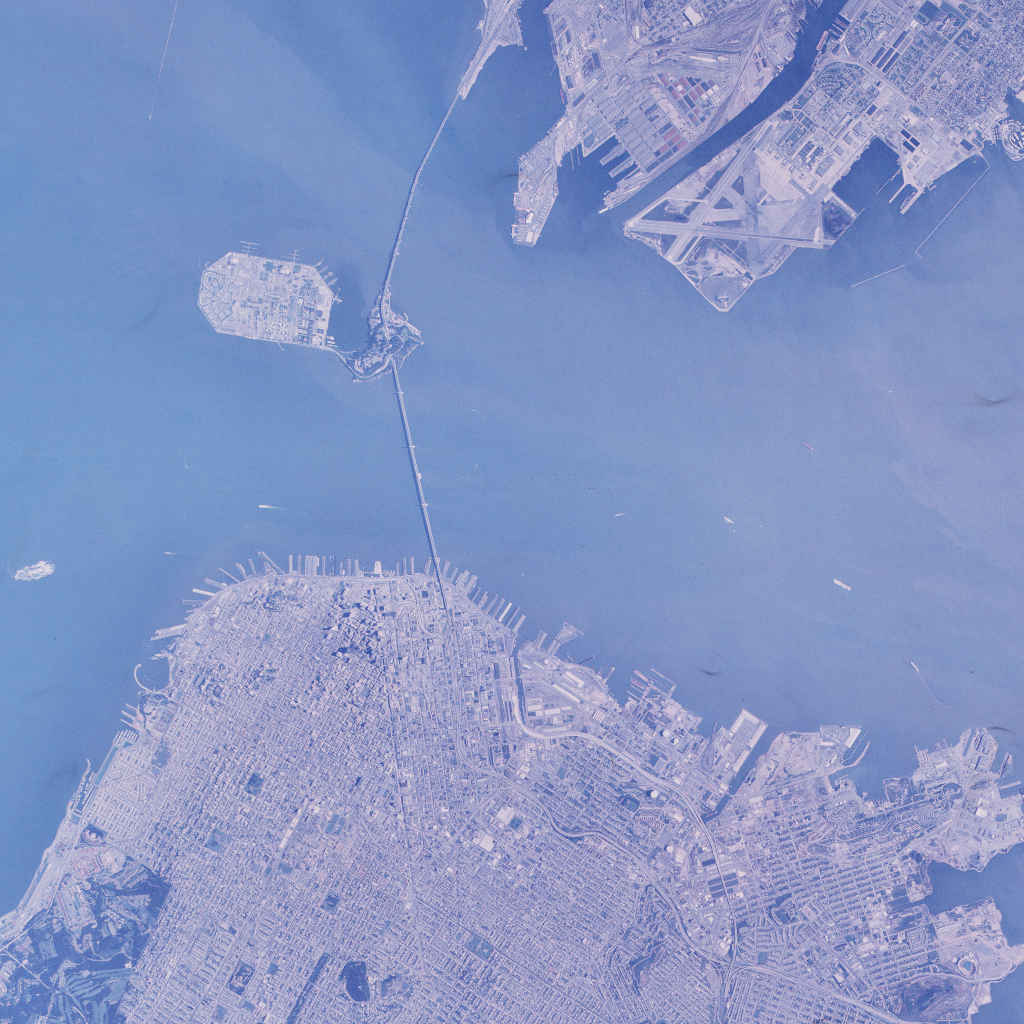
\includegraphics[width=4cm, height=4cm]{Figures/chap3/port1.jpg}
&

\includegraphics[width=4cm, height=4cm]{Figures/chap3/san_fransisco2.png}
&
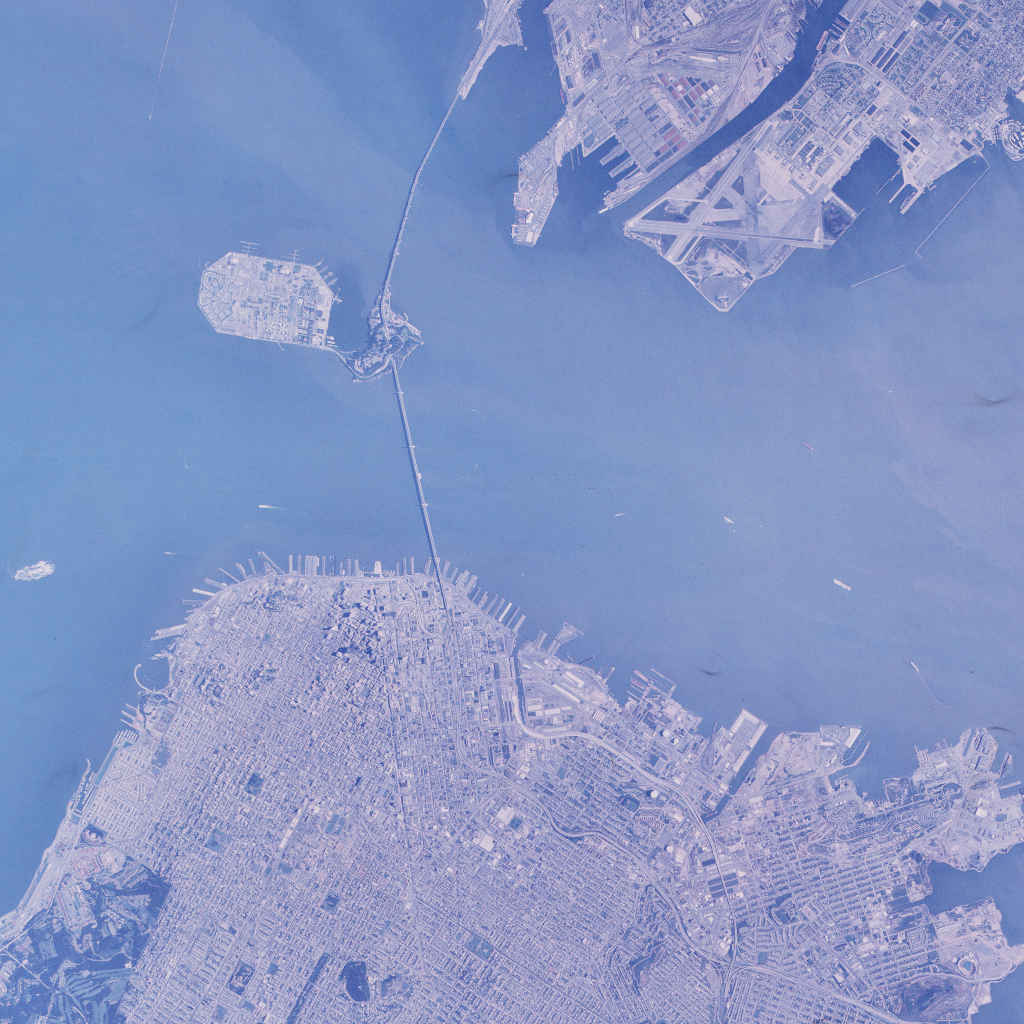
\includegraphics[width=4cm, height=4cm]{Figures/chap3/port1.jpg}
&

\includegraphics[width=4cm, height=4cm]{Figures/chap3/san_fransisco2.png}\\

\multicolumn{2}{c}{(c) San Fransisco}
&
\multicolumn{2}{c}{(d) Image aléatoire 2}

\end{tabular}
\caption[TraitementImage]{La segmentation d'images}

\end{figure}

\section{Conclusion}
\indent Dans ce dernier chapitre nous avons décrit l'interface de notre application et les détails de son fonctionnement. Nous avons fait une démonstration des deux différents modes d'utilisation : \textbf{automatique} et \textbf{contrôlé} (étape d'apprentissage) et avons aussi exposé les multiples options proposées dans ce dernier mode.\\
\indent Nous avons présenté une série de tests effectués sur différentes images aléatoirement construites et qui donnent des résultats satisfaisants et très prometteurs.\\
\indent Enfin, nous avons vu l'indépendance de cette méthode des formes utilisées pour la recherche et la reconnaissance des textures, qui représente un très grand avantage.
